% =============================================================================
% 5. Results -- target ~4 pp
% Lead with the headline plot. Each finding gets a short prose paragraph, a
% figure or table reference, and a Wilcoxon p-value where applicable.
% =============================================================================

\section{Results}
\label{sec:results}

\subsection{Primary Sweep}

SimPO is the only method that significantly beats the best ICL baseline at $n = 100$ on both datasets --- by 3.6 points on GoodReads ($p = 0.002$, paired Wilcoxon) and 5.9 points on Netflix ($p = 0.011$). Figure~\ref{fig:primary_curves} and Table~\ref{tab:primary_acc} show the full picture, and the same two-regime shape appears on both datasets. At $n \leq 10$ the trained methods sit at or below the frozen base model and the ICL baselines lead. The crossover lies between $n = 10$ and $n = 50$. From $n = 50$ onwards the trained methods overtake, with SimPO clear of the pack and IPO close behind.

\begin{figure}[h]
\centering
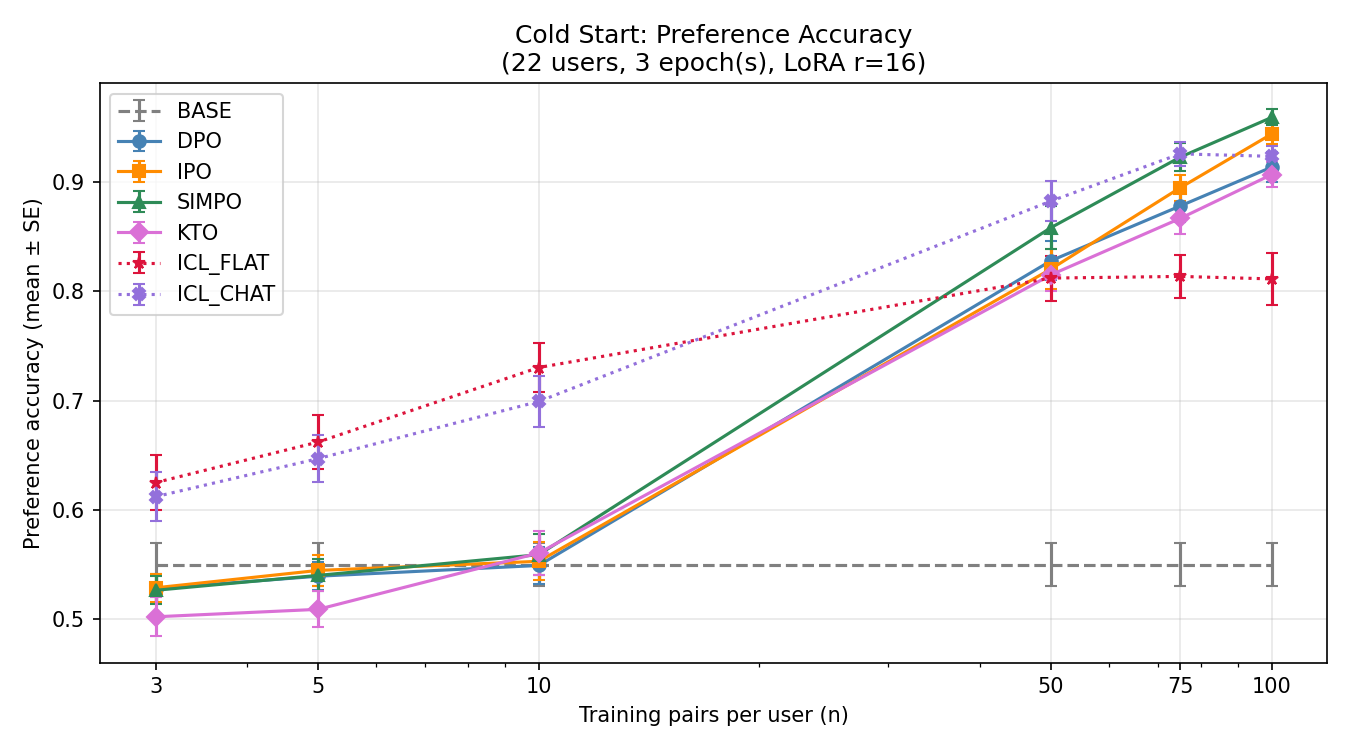
\includegraphics[width=0.48\textwidth]{images/primary_curves_goodreads.png}
\hfill
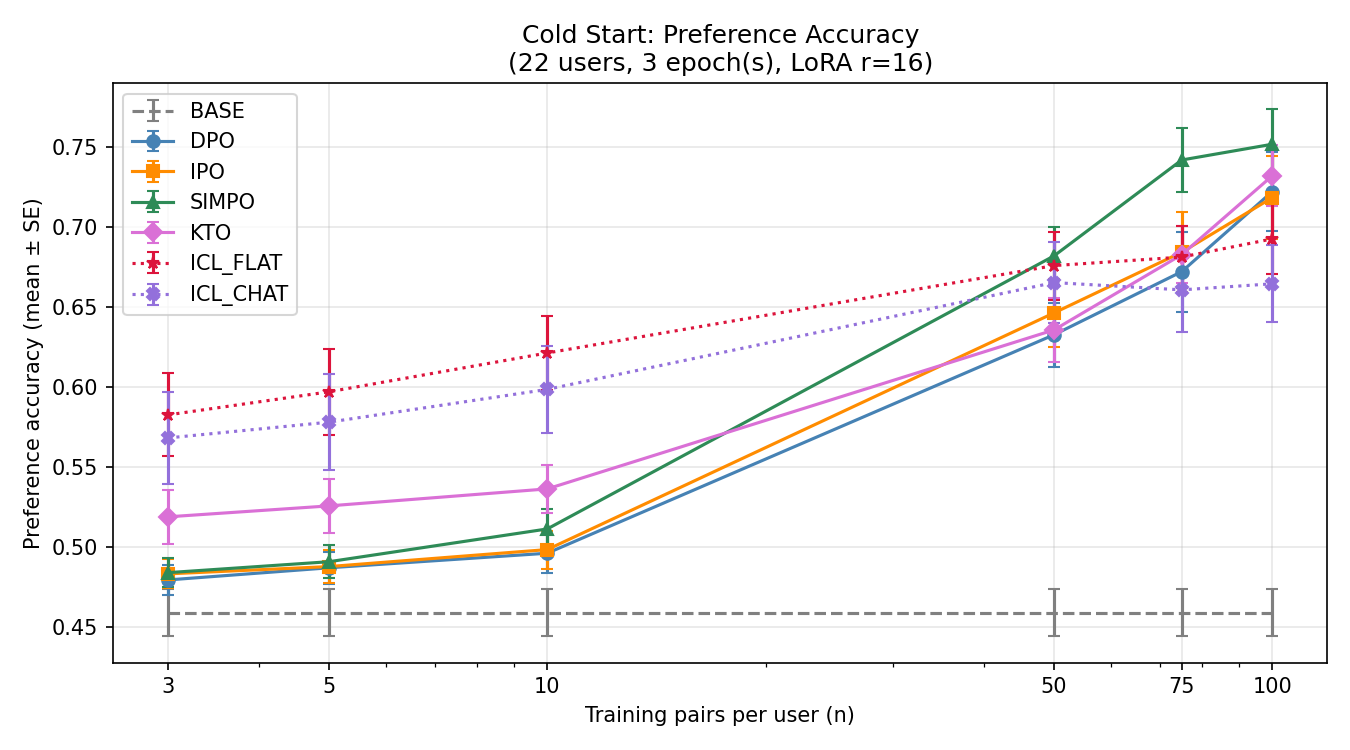
\includegraphics[width=0.48\textwidth]{images/primary_curves_netflix.png}
\caption{Held-out pairwise accuracy by training size $n$ and method. Left: GoodReads. Right: Netflix. Lines are means across users and seeds; shaded regions are $\pm 1$ standard error.}
\label{fig:primary_curves}
\end{figure}

\begin{table}[h]
\centering
\caption{Pairwise accuracy by method and training size. Bold marks the per-column best; $\dagger$ marks significant improvement over the best ICL baseline at the $0.05$ level (paired Wilcoxon at $n = 100$).}
\label{tab:primary_acc}
\begin{tabular}{lcccccc}
\toprule
\textbf{Method} & $n = 3$ & $n = 5$ & $n = 10$ & $n = 50$ & $n = 75$ & $n = 100$ \\
\midrule
\multicolumn{7}{l}{\textit{GoodReads}} \\
base                 & .550 & .550 & .550 & .550 & .550 & .550 \\
dpo                  & .528 & .539 & .549 & .828 & .878 & .914 \\
ipo                  & .529 & .545 & .553 & .820 & .895 & .944 \\
simpo                & .527 & .540 & .559 & .858 & .923 & \textbf{.959}$^\dagger$ \\
kto                  & .502 & .509 & .561 & .815 & .867 & .907 \\
icl\_flat            & \textbf{.625} & \textbf{.662} & \textbf{.730} & .812 & .814 & .811 \\
icl\_chat            & .612 & .647 & .699 & \textbf{.883} & \textbf{.926} & .923 \\
\midrule
\multicolumn{7}{l}{\textit{Netflix}} \\
base                 & .459 & .459 & .459 & .459 & .459 & .459 \\
dpo                  & .480 & .487 & .496 & .633 & .672 & .722 \\
ipo                  & .483 & .488 & .498 & .646 & .684 & .718 \\
simpo                & .484 & .491 & .511 & \textbf{.682} & \textbf{.742} & \textbf{.752}$^\dagger$ \\
kto                  & .519 & .526 & .536 & .636 & .683 & .732 \\
icl\_flat            & \textbf{.583} & \textbf{.597} & \textbf{.621} & .676 & .681 & .692 \\
icl\_chat            & .568 & .578 & .598 & .665 & .661 & .664 \\
\bottomrule
\end{tabular}
\end{table}

The per-user picture matches the means. SimPO wins on $14/22$ users on each dataset, against $7/22$ and $9/22$ for DPO, $10/22$ and $13/22$ for IPO, and $7/22$ and $14/22$ for KTO. The mean ranking and the per-user ranking agree, so the headline is not a few-user artefact.

Two dataset-level differences are worth flagging. The frozen base sits at $0.550$ on GoodReads and at $0.459$ on Netflix, so book titles already carry signal to the pretrained model while movie titles do not. And the ICL baselines swap order across datasets: \texttt{icl\_chat} leads on GoodReads, \texttt{icl\_flat} leads on Netflix. The chat-template advantage is real on books but not on films.

\subsection{Beyond the Cold-Start Cap}

Pushing $n$ from $100$ to $150$ on GoodReads pulls the trained methods toward ceiling and leaves the ICL plateau where it was. Mean accuracy at $n = 150$ is $0.983$ for SimPO, $0.958$ for IPO, $0.932$ for DPO and $0.920$ for KTO, against $0.806$ for \texttt{icl\_flat}. The pairwise ordering established at $n = 100$ in §5.1 is preserved, but the gap between SimPO and the rest of the trained methods narrows as everything approaches the upper bound of the evaluation.

\begin{table}[h]
\centering
\caption{GoodReads pairwise accuracy at $n = 150$, averaged across users and seeds.}
\label{tab:extended_acc}
\begin{tabular}{lc}
\toprule
\textbf{Method} & $n = 150$ \\
\midrule
dpo                 & .932 \\
ipo                 & .958 \\
simpo               & \textbf{.983} \\
kto                 & .920 \\
icl\_flat           & .806 \\
\bottomrule
\end{tabular}
\end{table}

Two notes qualify the comparison with §5.1. The extended sweep was run on a different draw of 22 GoodReads users from the same eligibility pool, with ten users in common with the primary sweep, so the $n = 150$ column is best read as a separate measurement on the same population rather than as a continuation of any individual user's curve. And \texttt{icl\_chat} is not reported here: at $n = 150$ the prompt-side context already exceeds what the chat template can carry under the $8{,}192$-token cap, and the method's accuracy collapses to a level that reflects truncation rather than model behaviour. The \texttt{icl\_flat} variant remains within its working range at this size.

\subsection{Per-User View}

The mean curves in §5.1 hide whether the gain is spread across users or concentrated in a few. Figure~\ref{fig:per_user} shows the full per-user grid: each panel is one user's learning curve under each method, on the same axes as Figure~\ref{fig:primary_curves}. Two facts emerge from the grid that are not visible in the means. No user is harmed by training at $n = 100$: on both datasets, the best trained method beats the frozen base model for every one of the twenty-two users. And no user is left stuck near chance: the worst best-method accuracy is $0.933$ on GoodReads and $0.600$ on Netflix.

\begin{figure}[h]
\centering
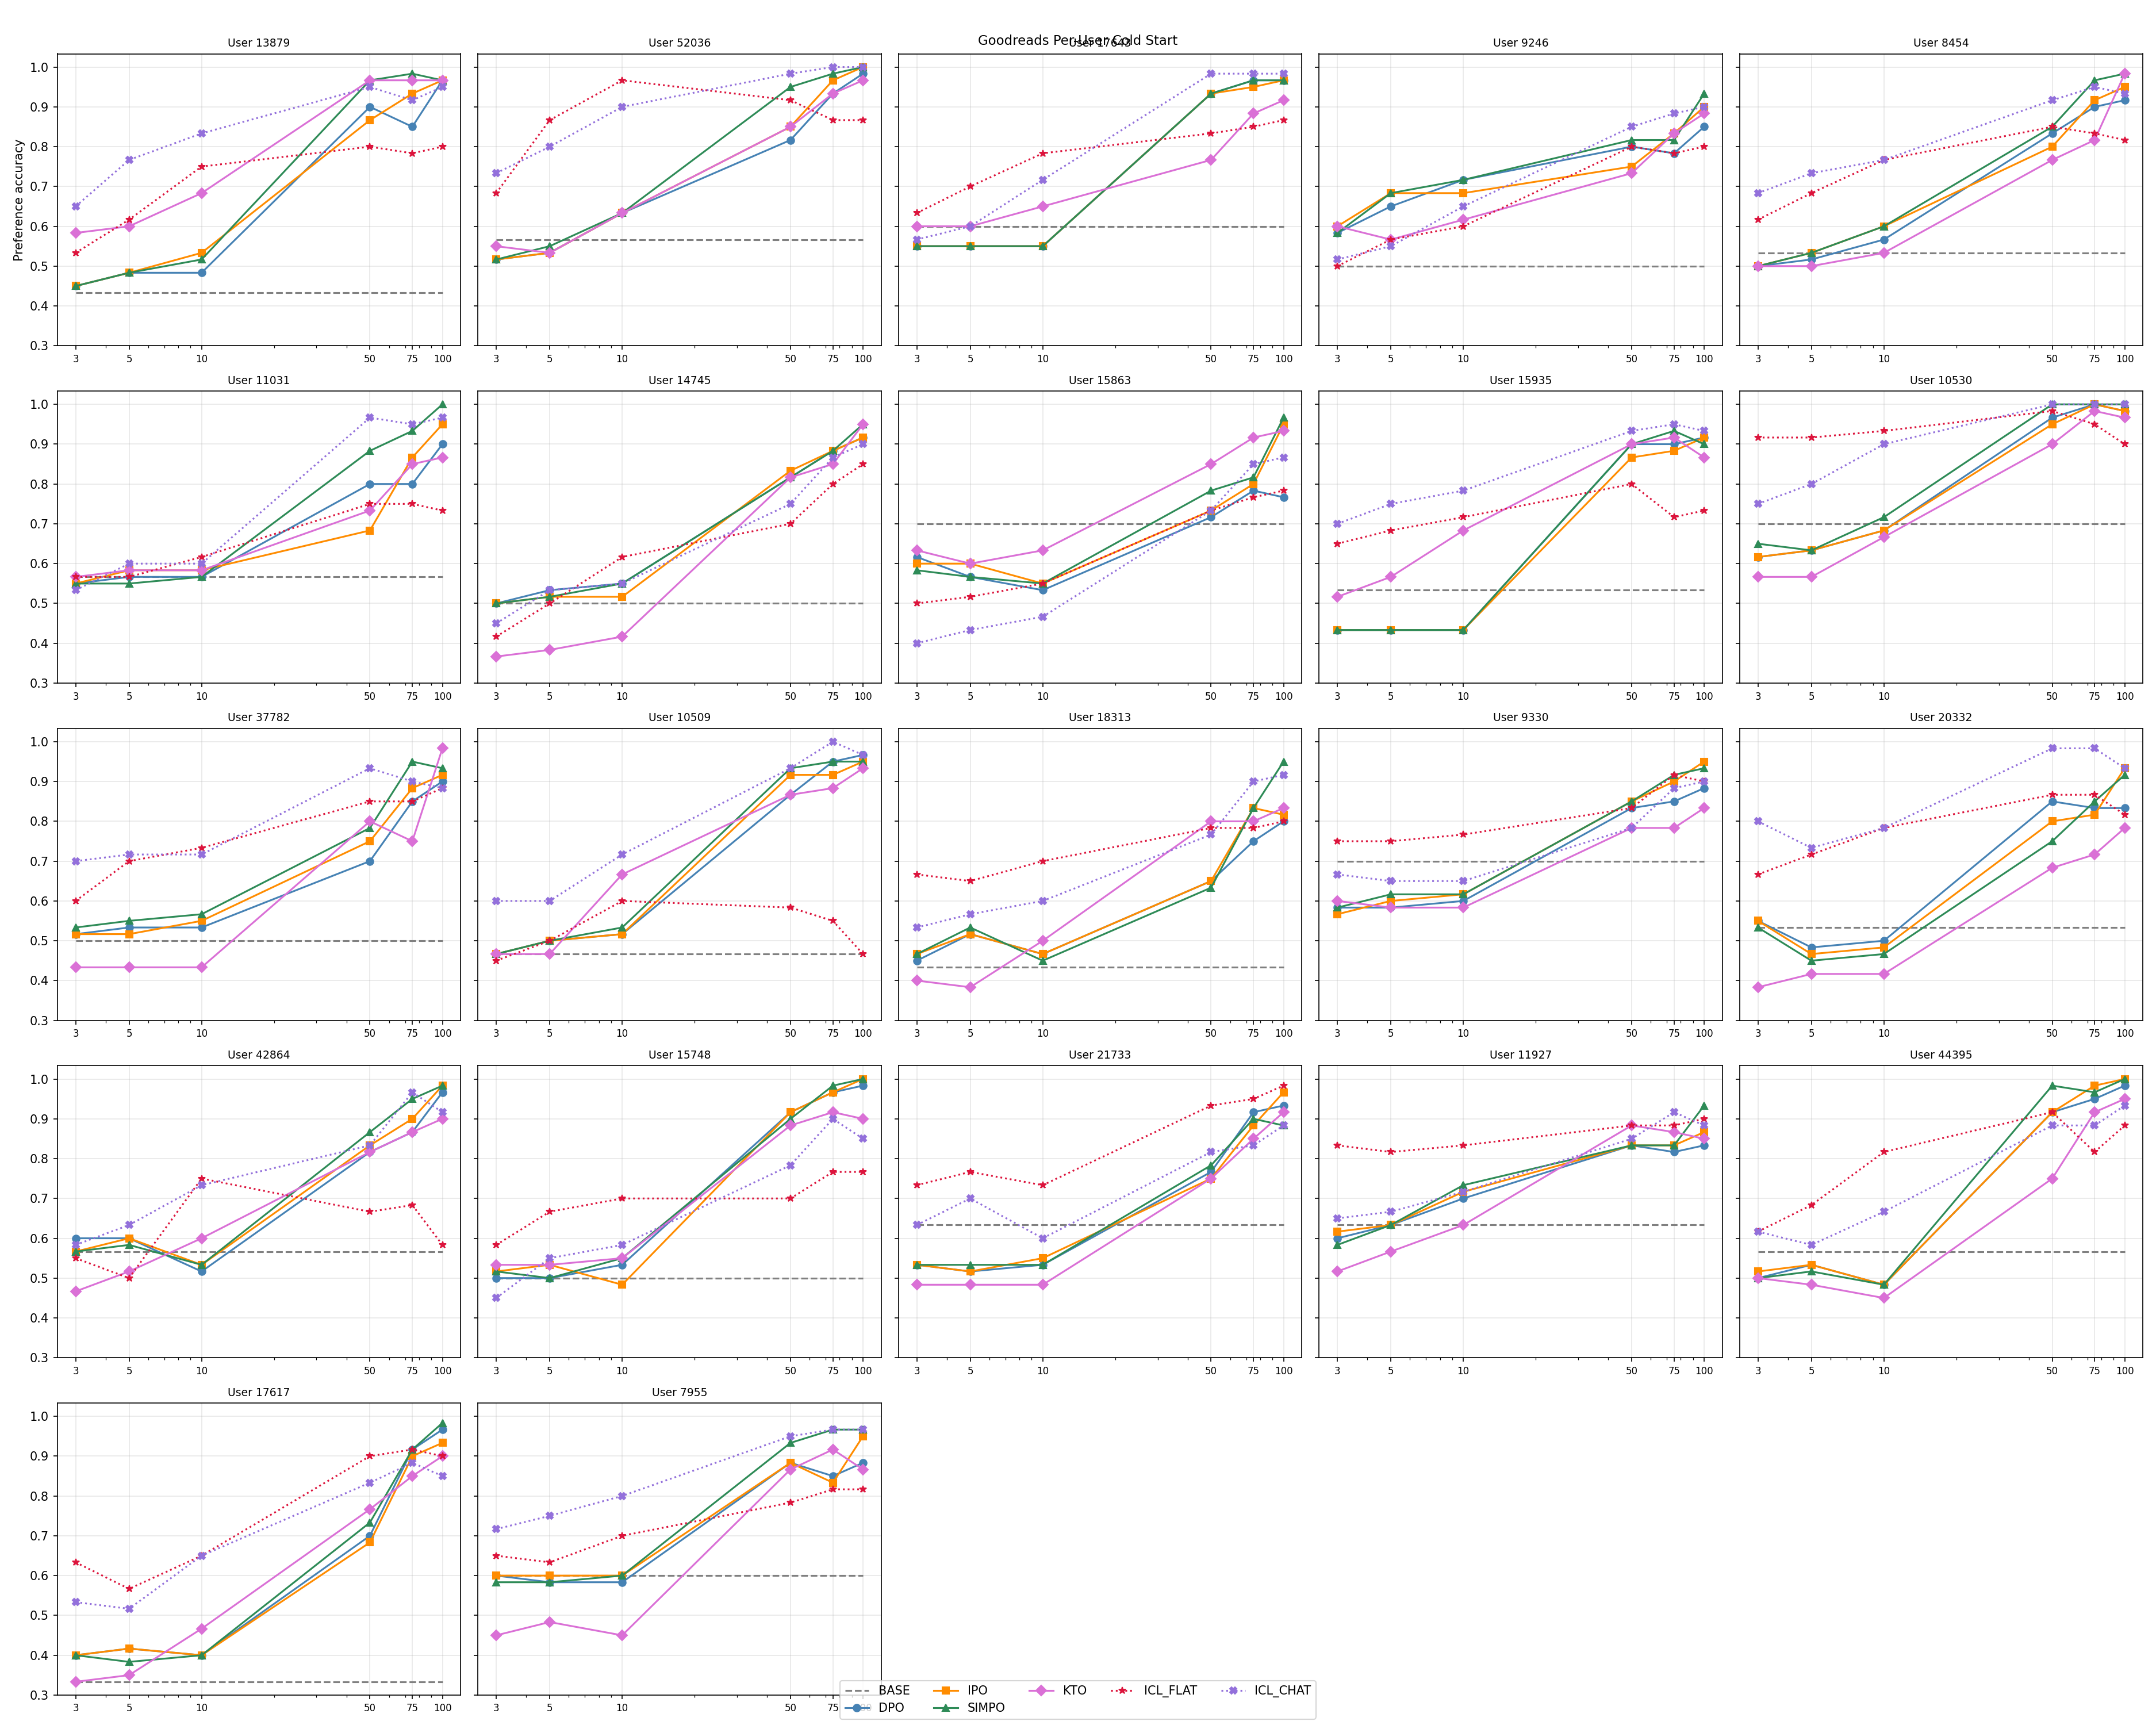
\includegraphics[width=0.48\textwidth]{images/per_user_goodreads.png}
\hfill
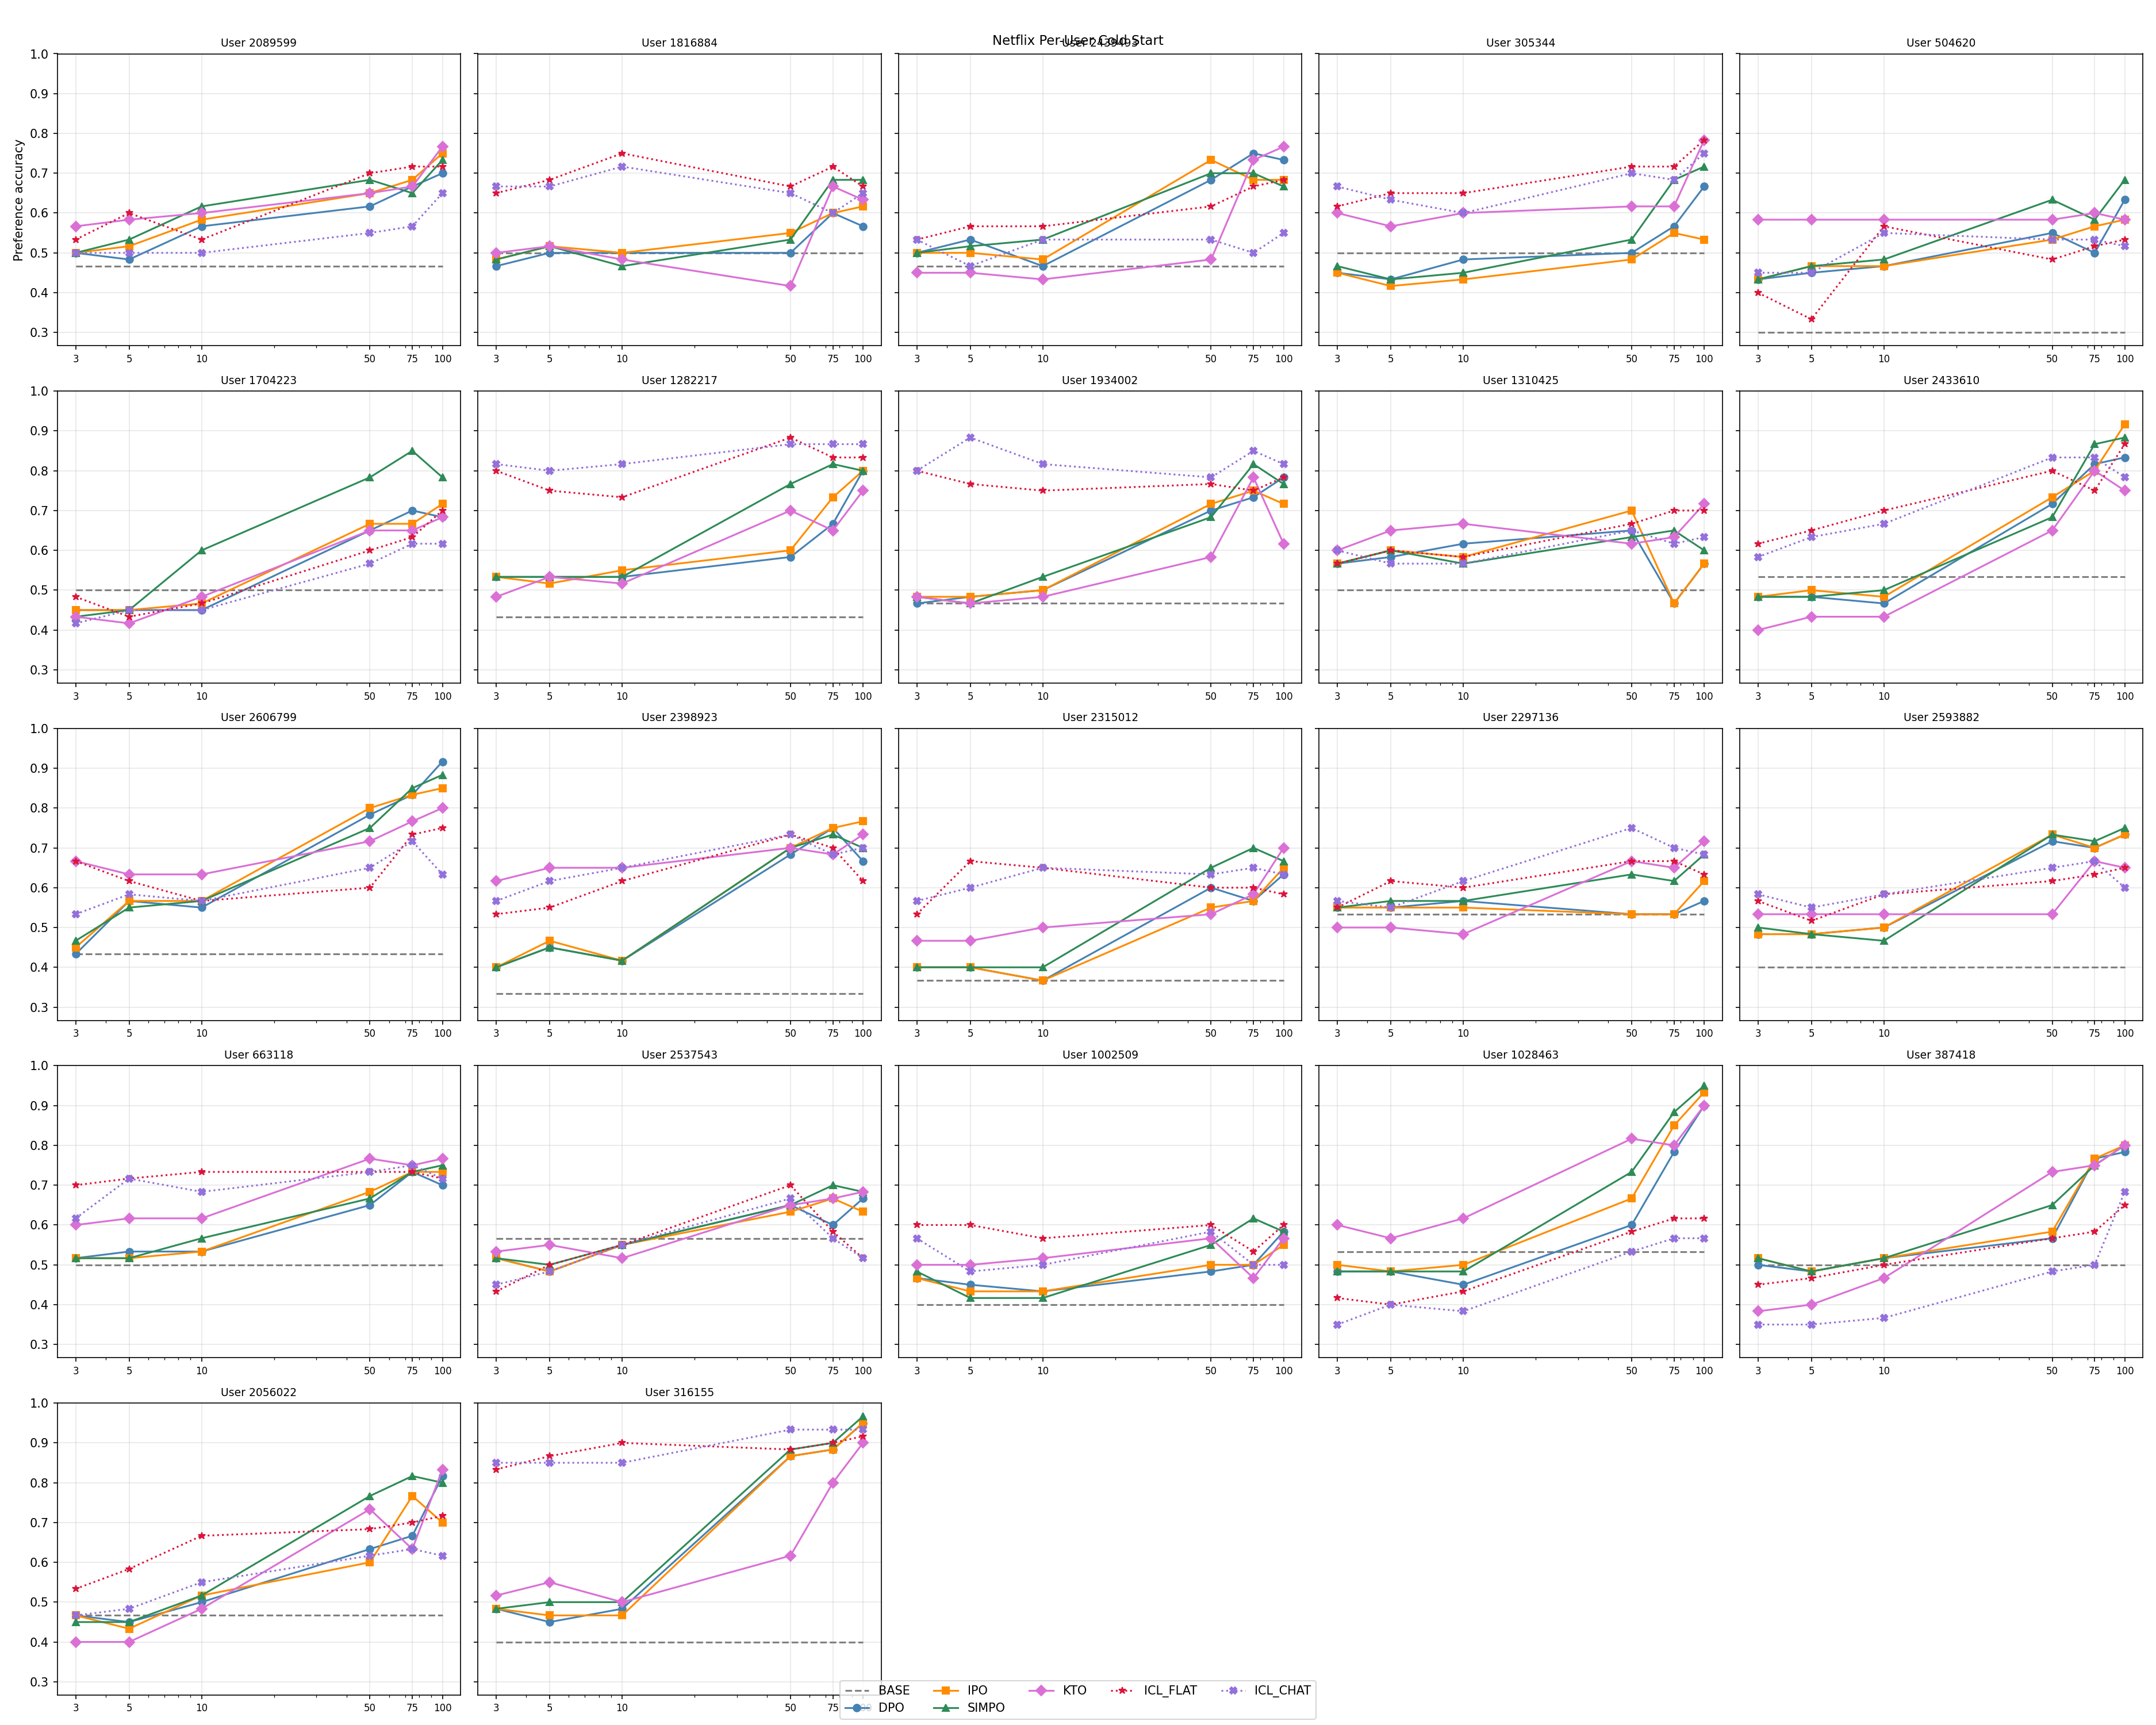
\includegraphics[width=0.48\textwidth]{images/per_user_netflix.png}
\caption{Per-user learning curves on GoodReads (left) and Netflix (right). Each panel is one user; lines are method means across the two seeds.}
\label{fig:per_user}
\end{figure}

\begin{table}[h]
\centering
\caption{Per-user picture at $n = 100$. Columns: spread of the best-method accuracy across the twenty-two users; users for whom no trained method exceeds the base; users where every method stays below $0.60$; outright per-user winner counts among the four trained methods and the two ICL baselines.}
\label{tab:per_user}
\begin{tabular}{lcc}
\toprule
 & \textbf{GoodReads} & \textbf{Netflix} \\
\midrule
Best-method accuracy range          & $[.933,\ 1.000]$ & $[.600,\ .967]$ \\
Users hurt by training              & $0/22$           & $0/22$ \\
Users with no method above $0.60$   & $0/22$           & $0/22$ \\
\midrule
Outright winners (out of $22$) &  & \\
\quad simpo                          & $10$              & $7$ \\
\quad ipo                            & $6$               & $3$ \\
\quad dpo                            & $2$               & $2$ \\
\quad kto                            & $1$               & $7$ \\
\quad \texttt{icl\_chat}             & $2$               & $2$ \\
\quad \texttt{icl\_flat}             & $1$               & $1$ \\
\bottomrule
\end{tabular}
\end{table}

Two things qualify the §5.1 ranking once the per-user picture is in view. SimPO wins the mean comparison and the most users on both datasets, but it is not the per-user winner for $12/22$ GoodReads users and $15/22$ Netflix users --- for those, another trained method matches or exceeds it. The per-user grid also shows that the cold-start advantage of ICL is itself heterogeneous: at $n = 10$, the best ICL baseline beats the best trained method for $20/22$ GoodReads users but only $13/22$ Netflix users. The pattern in the means therefore holds at the user level, but with meaningful per-user variation that any deployment based on these results would need to plan for.